\UseRawInputEncoding
\documentclass[12pt]{article}
\title{ECE C143A Homework 3}
\usepackage{subcaption}
\author{Lawrence Liu}
\usepackage{graphicx}
\usepackage{amsmath}
\usepackage{bm}
\usepackage{pdfpages}
\newcommand{\Laplace}{\mathscr{L}}
\setlength{\parskip}{\baselineskip}%
\setlength{\parindent}{0pt}%
\usepackage{xcolor}
\usepackage{listings}
\definecolor{backcolour}{rgb}{0.95,0.95,0.92}
\usepackage{amssymb}
\lstdefinestyle{mystyle}{
    backgroundcolor=\color{backcolour}}
\lstset{style=mystyle}

\begin{document}
\maketitle
\section*{Problem 1}
\subsection*{(a)}
We have
\begin{align*}
    L&=\Pi_{i=0}P(\textbf{x}_i,t_i)\\
    &=\Pi_{i=0}P(t_i)P(\textbf{x}_i|t_i)
\end{align*}
let $P(t_i=j)=P(C_j)$, therefore we have
\begin{align*}
    L&=\Pi_{i\in C_1}P(C_1)P(\textbf{x}_i|C_1)\dots \Pi_{i\in C_k}P(C_k)P(\textbf{x}_i|C_k)\\
    \log(L)&=\sum_{i=1}^{k}N_i\log(P(c_i))+\sum_{j\in C_1}\log(P(\textbf{x}_j|C_1))+
                    \dots+\sum_{j\in C_k}\log(P(\textbf{x}_j|C_k))
\end{align*}
We have
$$P(\textbf{x}_j|C_k)=(2\pi\det(\Sigma_k))^{-\frac{1}{2}}\exp(-\frac{1}{2}(\textbf{x}_j-\mu_k)^T\Sigma_k^{-1}(\textbf{x}_j-\mu_k))$$
$$\log(P(\textbf{x}_j|C_k))=-\frac{1}{2}\log(2\pi\det(\Sigma_k))-\frac{1}{2}(\textbf{x}_j-\mu_k)^T\Sigma_k^{-1}(\textbf{x}_j-\mu_k)$$
In order to find the maximum likelihood estimator $\mu_k$ we find the values of $\mu_k$ such that $\frac{\partial \log{L}}{\partial \mu_k}=0$,
Therefore we have
\begin{align*}
\frac{\partial \log{L}}{\partial \mu_k}&=\sum_{j\in C_k}-\frac{1}{2}\frac{\partial}{\partial\mu_k}(\textbf{x}_j-\mu_k)^T\Sigma_k^{-1}(\textbf{x}_j-\mu_k)
&=-\frac{1}{2}\sum_{j\in C_k}(\Sigma_k+\Sigma_k^{T})(\textbf{x}_k-\mu_k)\\
&=-\frac{1}{2}(\Sigma_k+\Sigma_k^{T})\sum_{j\in C_k}\textbf{x}_k-\mu_k
\end{align*}
therefore we have that in order for $\frac{\partial \log{L}}{\partial \mu_k}=0$,
$$\sum_{j\in C_k}\textbf{x}_k-\mu_k=0$$
$$\boxed{\mu_k=\frac{1}{N_k}\sum_{j\in C_k}\textbf{x}_k}$$
Likewise, the maximum likelihood estimator of $\Sigma_k$ is the values such that $\frac{\partial \log{L}}{\partial \Sigma_k}=0$, this is equivalent to finding the values of
$\Sigma_k^{-1}$ such that $\frac{\partial \log{L}}{\partial \Sigma_k^{-1}}=0$
\begin{align*}
\frac{\partial \log{L}}{\partial \Sigma_k^{-1}}&=0\\
\frac{1}{2}\frac{\partial N_k\log(2\pi\det(\Sigma_k))+\sum_{i\in k}(\textbf{x}_j-\mu_k)^T\Sigma_k^{-1}(\textbf{x}_j-\mu_k)}{\partial \Sigma_k^{-1}}&=0
\end{align*}
We have
\begin{align*}
    \frac{\partial\log(2\pi\det(\Sigma_k))}{\partial \Sigma_k^{-1}}&=\frac{\partial\log(\det(\Sigma_k))}{\partial \Sigma_k^{-1}}\\
    &=\frac{1}{\det(\Sigma_k)}\frac{\partial \det(\Sigma_k)}{\partial \Sigma_k^{-1}}\\
    &=\frac{1}{\det(\Sigma_k)}(-\det(\Sigma_k))\Sigma_k^T\\
    &=-\Sigma_k^T
\end{align*}
Furthermore we have
\begin{align*}
    \frac{\partial(\textbf{x}_j-\mu_k)^T\Sigma_k^{-1}(\textbf{x}_j-\mu_k)}{\partial \Sigma_k^{-1}}&=(\textbf{x}_j-\mu_k)^T(\textbf{x}_j-\mu_k)
\end{align*}
Therefore we have
\begin{align*}
    0&=\frac{\partial \log{L}}{\partial \Sigma_k^{-1}}=-N_k\Sigma_k^T+\sum_{i\in C_k}(\textbf{x}_j-\mu_k)^T(\textbf{x}_j-\mu_k)\\
    N_k\Sigma_k^T&=\sum_{i\in C_k}(\textbf{x}_j-\mu_k)^T(\textbf{x}_j-\mu_k)\\
    \Sigma_k&=\boxed{\frac{1}{N_k}\sum_{i\in C_k}(\textbf{x}_j-\mu_k)(\textbf{x}_j-\mu_k)^T}
\end{align*}
And to find the maximum likelihood estimator for $P(C_i)$ we must find the value of $P(C_i)$ for any $i\in k$ such that 
$\sum_{j \in k} N_j\log(p(C_j))$ is maximized, since $\sum_{i\in K}p(C_i)=1$, we have $\sum_{j \in k} N_j\log(p(C_j))=\sum_{j \in k} N_j\log(p(C_j))+\lambda(\sum_{i\in K}p(C_j)-1)$
Therefore taking the derivative of each with respect to $P(C_i)$ for any $i\in k$ we get
\begin{align*}
    \frac{\partial }{\partial P(C_1)}\sum_{j \in k} N_jp(C_j)+\lambda(\sum_{i\in K}p(C_i)-1)&=\frac{N_j}{C_j}+\lambda=0\\
    \vdots \\
    \frac{\partial }{\partial P(C_k)}\sum_{j \in k} N_jp(C_j)+\lambda(\sum_{i\in K}p(C_i)-1)&=\frac{N_k}{C_k}+\lambda=0\\
    \frac{\partial }{\partial \lambda}\sum_{j \in k} N_jp(C_j)+\lambda(\sum_{i\in K}p(C_i)-1)&=\sum_{i\in K}p(C_i)=1
\end{align*}
Solving these we get that $p(C_k)=\boxed{\frac{N_k}{N}}$

\subsection*{(b)}
We have
\begin{align*}
    L&=\Pi_{i=0}P(\textbf{x}_i,t_i)\\
    &=\Pi_{i=0}P(t_i)P(\textbf{x}_i|t_i)
\end{align*}
let $P(t_i=j)=P(C_j)$, therefore we have
\begin{align*}
    L&=\Pi_{i\in C_1}P(C_1)P(\textbf{x}_i|C_1)\dots \Pi_{i\in C_k}P(C_k)P(\textbf{x}_i|C_k)\\
    \log(L)&=\sum_{i=1}^{k}N_i\log(P(c_i))+\sum_{j\in C_1}\log(P(\textbf{x}_j|C_1))+
                    \dots+\sum_{j\in C_k}\log(P(\textbf{x}_j|C_k))
\end{align*}
We have
$$P(\textbf{x}_j|C_k)=\Pi_{i=1}^{D}P(x_i|C_k)$$
where
$$P(x_i|C_k)=\text{Poisson}(\lambda_{ik})=\frac{\lambda_{ik}^{x_i}e^{-\lambda_{ik}}}{x_i!}$$
Therefore we have
\begin{align*}
    log(P(\textbf{x}_j|C_k))&=\sum_{i=1}^{D}\log\left(\frac{\lambda_{ik}^{x_i}e^{-\lambda_{ik}}}{x_i!}\right)\\
    &=\sum_{i=1}^{D}\left(x_i\log(\lambda_{ik})-\lambda_{ik}-\log(x_i!)\right)
\end{align*}
the maximum likelihood estimator of $\lambda_{ik}$ is the values such that $\frac{\partial \log{L}}{\partial \lambda_{ik}}=0$, we have
\begin{align*}
    \frac{\partial}{\partial \lambda_{ik}}\log(L)&=\frac{\partial}{\partial \lambda_{ik}}\sum_{i=1}^{k}N_i\log(P(c_i))+\frac{\partial}{\partial \lambda_{ik}}\sum_{j\in C_1}\log(P(\textbf{x}_j|C_1))+
                    \dots+\frac{\partial}{\partial \lambda_{ik}}\sum_{j\in C_k}\log(P(\textbf{x}_j|C_k))\\
                    &=\frac{\partial}{\partial \lambda_{ik}}\sum_{j\in C_k}\log(P(\textbf{x}_j|C_k))
\end{align*}
\begin{align*}
    \frac{\partial}{\partial \lambda_{ik}}\log(P(\textbf{x}_j|C_k))&=\frac{\partial}{\partial \lambda_{ik}}\left(x_i\log(\lambda_{ik})-\lambda_{ik}-\log(x_i!)\right)\\
    &=\frac{x_i}{\lambda_{ik}}-1
\end{align*}
Therefore we have
\begin{align*}
    0&=\frac{\partial}{\partial \lambda_{ik}}\log(L)\\
    0&=\sum_{j\in C_k}\frac{x_ji}{\lambda_{ik}}-1\\
    N_k\lambda_{ik}&=\sum_{j\in C_k}x_ji\\
    \lambda_{ik}&=\boxed{\frac{1}{N_k}\sum_{j\in C_k}x_ji}
\end{align*}
And to find the maximum likelihood estimator for $P(C_i)$ we must find the value of $P(C_i)$ for any $i\in k$ such that 
$\sum_{j \in k} N_j\log(p(C_j))$ is maximized, since $\sum_{i\in K}p(C_i)=1$, we have $\sum_{j \in k} N_j\log(p(C_j))=\sum_{j \in k} N_j\log(p(C_j))+\lambda(\sum_{i\in K}p(C_j)-1)$
Therefore taking the derivative of each with respect to $P(C_i)$ for any $i\in k$ we get
\begin{align*}
    \frac{\partial }{\partial P(C_1)}\sum_{j \in k} N_jp(C_j)+\lambda(\sum_{i\in K}p(C_i)-1)&=\frac{N_j}{C_j}+\lambda=0\\
    \vdots \\
    \frac{\partial }{\partial P(C_k)}\sum_{j \in k} N_jp(C_j)+\lambda(\sum_{i\in K}p(C_i)-1)&=\frac{N_k}{C_k}+\lambda=0\\
    \frac{\partial }{\partial \lambda}\sum_{j \in k} N_jp(C_j)+\lambda(\sum_{i\in K}p(C_i)-1)&=\sum_{i\in K}p(C_i)=1
\end{align*}
Solving these we get that $p(C_k)=\boxed{\frac{N_k}{N}}$
\section*{Problem 2}
\subsection*{(a)}
We have that the decision boundary is all values of $\textbf{x}$ such that 
$$P(\textbf{x},C_1)=P(\textbf{x},C_2)$$
Therefore we must have 
\begin{align*}
    P(C_1)P(\textbf{x}|C_1)&=P(C_1)P(\textbf{x}|C_2)\\
    log(P(C_1))-\frac{1}{2}\log(2\pi\det(\Sigma_1))-\frac{1}{2}(\textbf{x}-\mu_1)^T\Sigma_1^{-1}(\textbf{x}-\mu_1)&=\\
    log(P(C_2))-\frac{1}{2}\log(2\pi\det(\Sigma_2))-\frac{1}{2}(\textbf{x}-\mu_2)^T\Sigma_2^{-1}(\textbf{x}-\mu_2)
\end{align*}
Therefore the decision boundary is
$$\boxed{\textbf{x}^TA\textbf{x}+B\textbf{x}+C=0}$$
where
$$A=\frac{1}{2}(\Sigma_1^{-1}-\Sigma_2^{-1})$$
$$B=\mu_2^T\Sigma_2^{-1}-\mu_1^T\Sigma_1^{-1}$$
\begin{multline*}
    C=\log(P(C_2))-\log(P(C_1))+\frac{1}{2}\log(2\pi\det(\Sigma_1))-\frac{1}{2}\log(2\pi\det(\Sigma_2))\\
+\frac{1}{2}\mu_1^T\Sigma_1^{-1}\mu_1-\frac{1}{2}\mu_2^T\Sigma_2^{-1}\mu_2
\end{multline*}
This is not linear, therefore the linear decision boundary is not linear
\subsection*{(b)}
We have that the decision boundary is all values of $\textbf{x}$ such that 
$$P(\textbf{x},C_1)=P(\textbf{x},C_2)$$
Therefore we must have 
\begin{align*}
    P(C_1)P(\textbf{x}|C_1)&=P(C_1)P(\textbf{x}|C_2)\\
    log(P(C_1))+\sum_{i=1}^{D}\left(x_i\log(\lambda_{i1})-\lambda_{i1}-\log(x_i!)\right)&=log(P(C_2))+\sum_{i=1}^{D}\left(x_i\log(\lambda_{i2})-\lambda_{i2}-\log(x_i!)\right)
\end{align*}
let $\bm{\lambda}_1=\begin{bmatrix}
    \lambda_{11} \\
    \vdots \\
    \lambda_{D1}
  \end{bmatrix}$, and $\bm{\lambda}_2=\begin{bmatrix}
    \lambda_{12} \\
    \vdots \\
    \lambda_{D2}
  \end{bmatrix}$, we have
\begin{align*}
    \log(P(C_1))-\sum_{i=1}^{D}\lambda_{i1}+\log(\bm{\lambda}_1)^T\textbf{x}&=
    \log(P(C_2))-\sum_{i=1}^{D}\lambda_{i2}+\log(\bm{\lambda}_2)^T\textbf{x}
\end{align*}
Therefore the decision boundary is,
$$\boxed{\log(P(C_1))-\sum_{i=1}^{D}\lambda_{i1}-\log(P(C_2))+\sum_{i=1}^{D}\lambda_{i2}=
(\log(\bm{\lambda}_2)^T-\log(\bm{\lambda}_1)^T)\textbf{x}}$$
Therefore there will be a linear decision boundary.
%\section*{Problem 3}
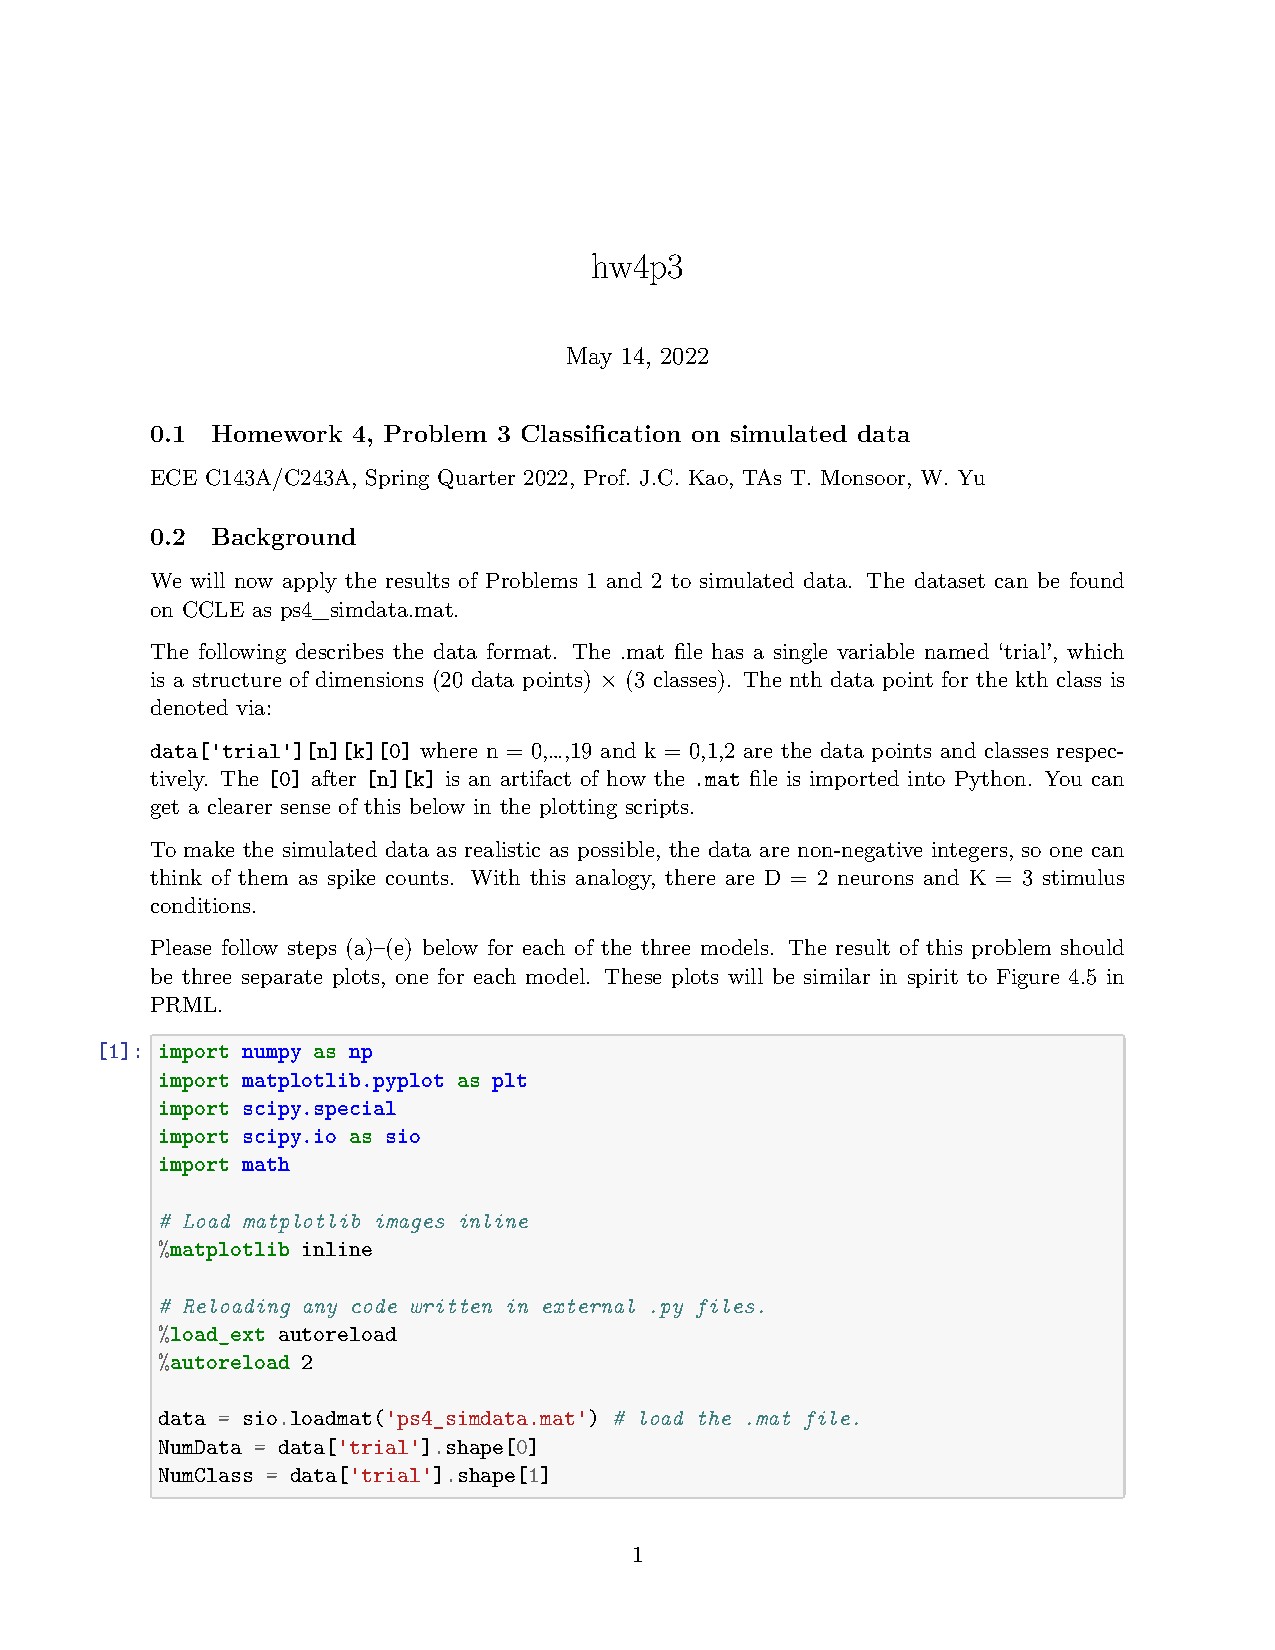
\includepdf[pages=-]{hw4p3.pdf}
%\section*{Problem 4}
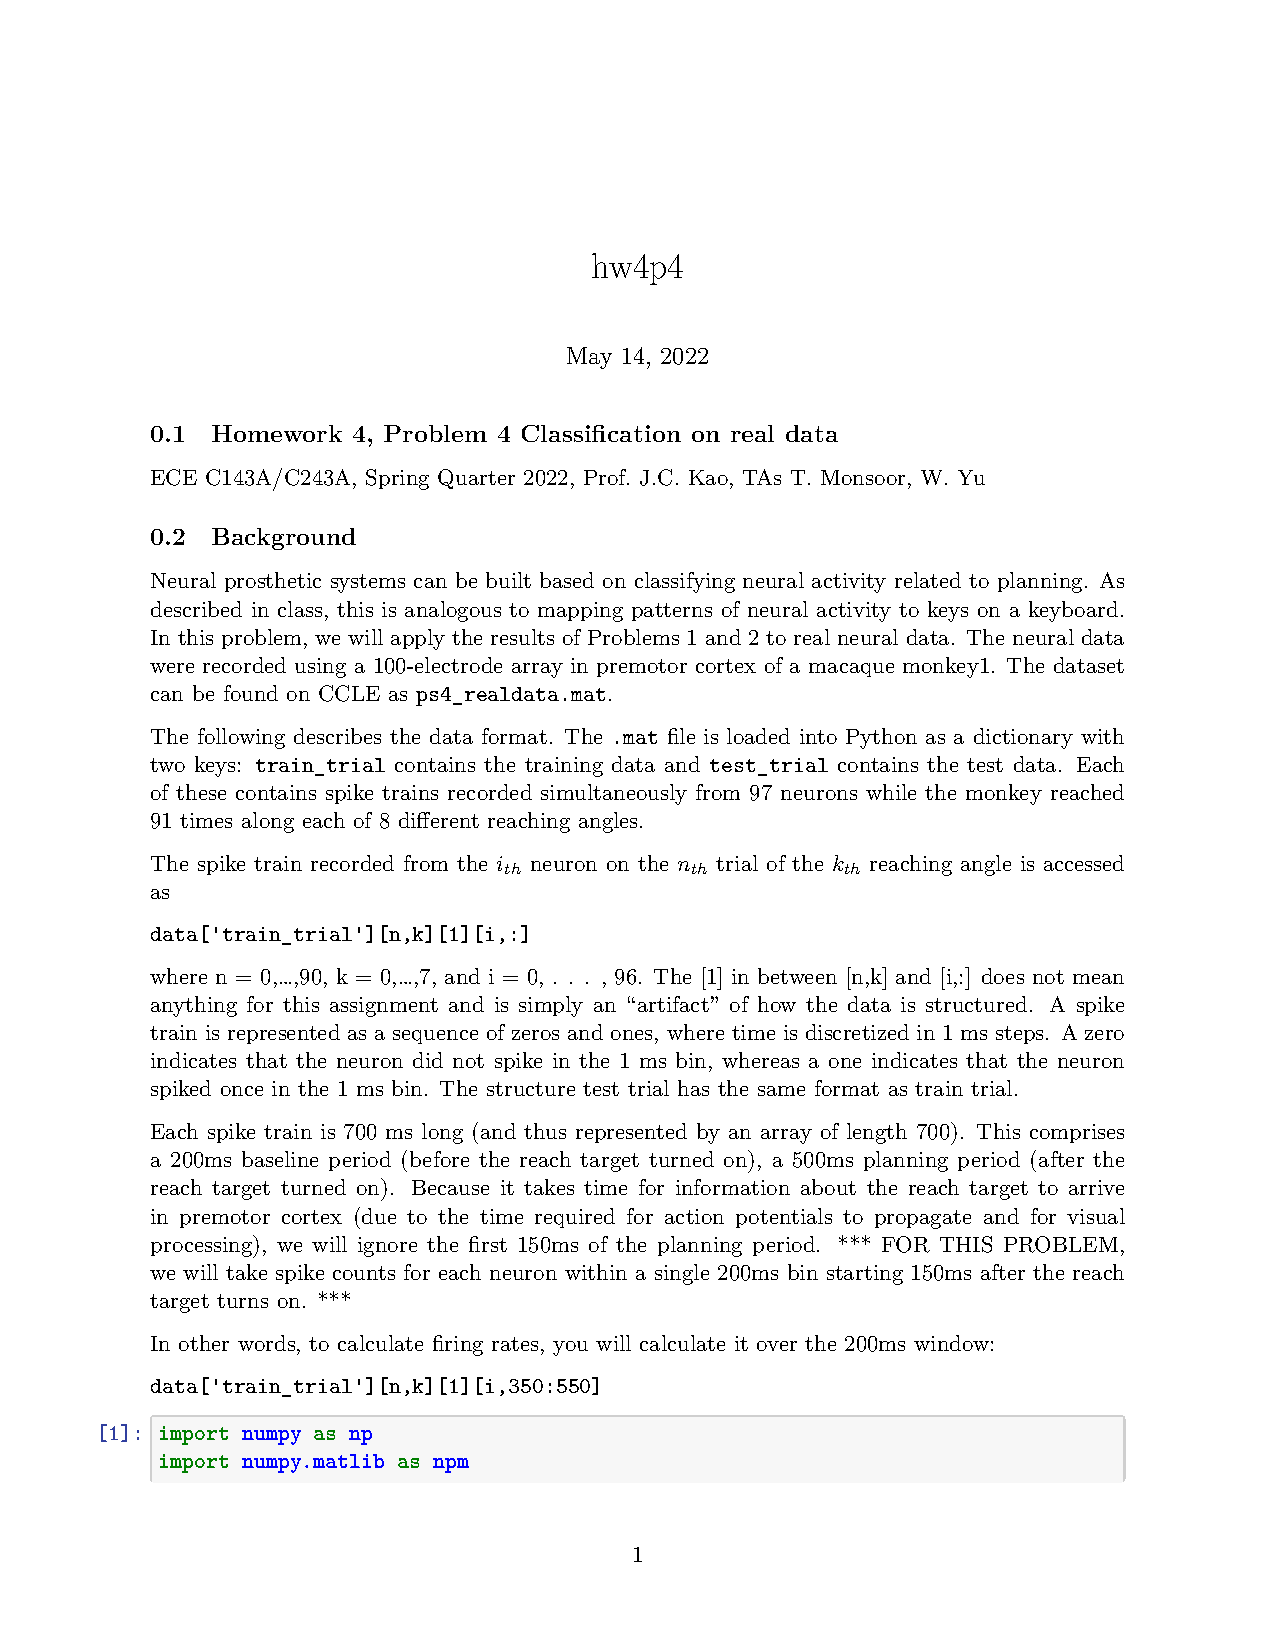
\includepdf[pages=-]{hw4p4.pdf}
\end{document}